\documentclass[a4paper,11pt,titlepage]{jarticle}
\usepackage[dvipdfmx]{graphicx} %pパッケージ
\usepackage{listings}
\usepackage{amsmath}
\usepackage{here}
\usepackage{url} 

\title{画像処理レポート1} %タイトル欄
\author{学籍番号:175769F \\ 氏名:新城 巧也}
\date{令和1年年10月27日}
\begin{document}
\maketitle
\tableofcontents %目次
\clearpage

\section{開発環境構築}
\subsection{Pythonの構築}
今回は、Homebrewでinstallする方法を下記のように示す。

\begin{verbatim}
$ brew install python 
\end{verbatim}
\begin{verbatim}
 また、zshなら~/.zshrcに、bashなら~/.bash_profileに以下のようなPATHを記述する。

export PATH=/usr/local/bin:$PATH

最後に$ which pythonのコマンドを実行すると/usr/local/bin/pythonと出力される。
\end{verbatim}
\subsection{Pillowの構築}

\begin{verbatim}
 Pillowをinstallするには、pipコマンドを使う方が一般的である。pipコマンドとは、PyPIと呼ばれるライブラリを管理するところから必要なライブラリをinstallすることができるコマンドのことである。下記に示す方法でinstallができる。

$ pip3 install pillow
\end{verbatim}

\subsection{NumPyの構築}
\begin{verbatim}
 NumPyのinstallもPillowと同様にpipを用いる。

 $ pip3 install numpy
\end{verbatim}
\section{画像の表示課題}
\subsection{プログラムコード}
実際に画像を表示させるコードをListing1に示す。
\lstinputlisting[numbers=left,breaklines=true,basicstyle=\ttfamily
\footnotesize,frame=single,caption=画像を表示させるコード,label=ex3]
{plot.py}\label{ex3}

\subsection{実行結果}
実行結果を図\ref{ex1}に示す。
\begin{figure}[H]
	\centering
	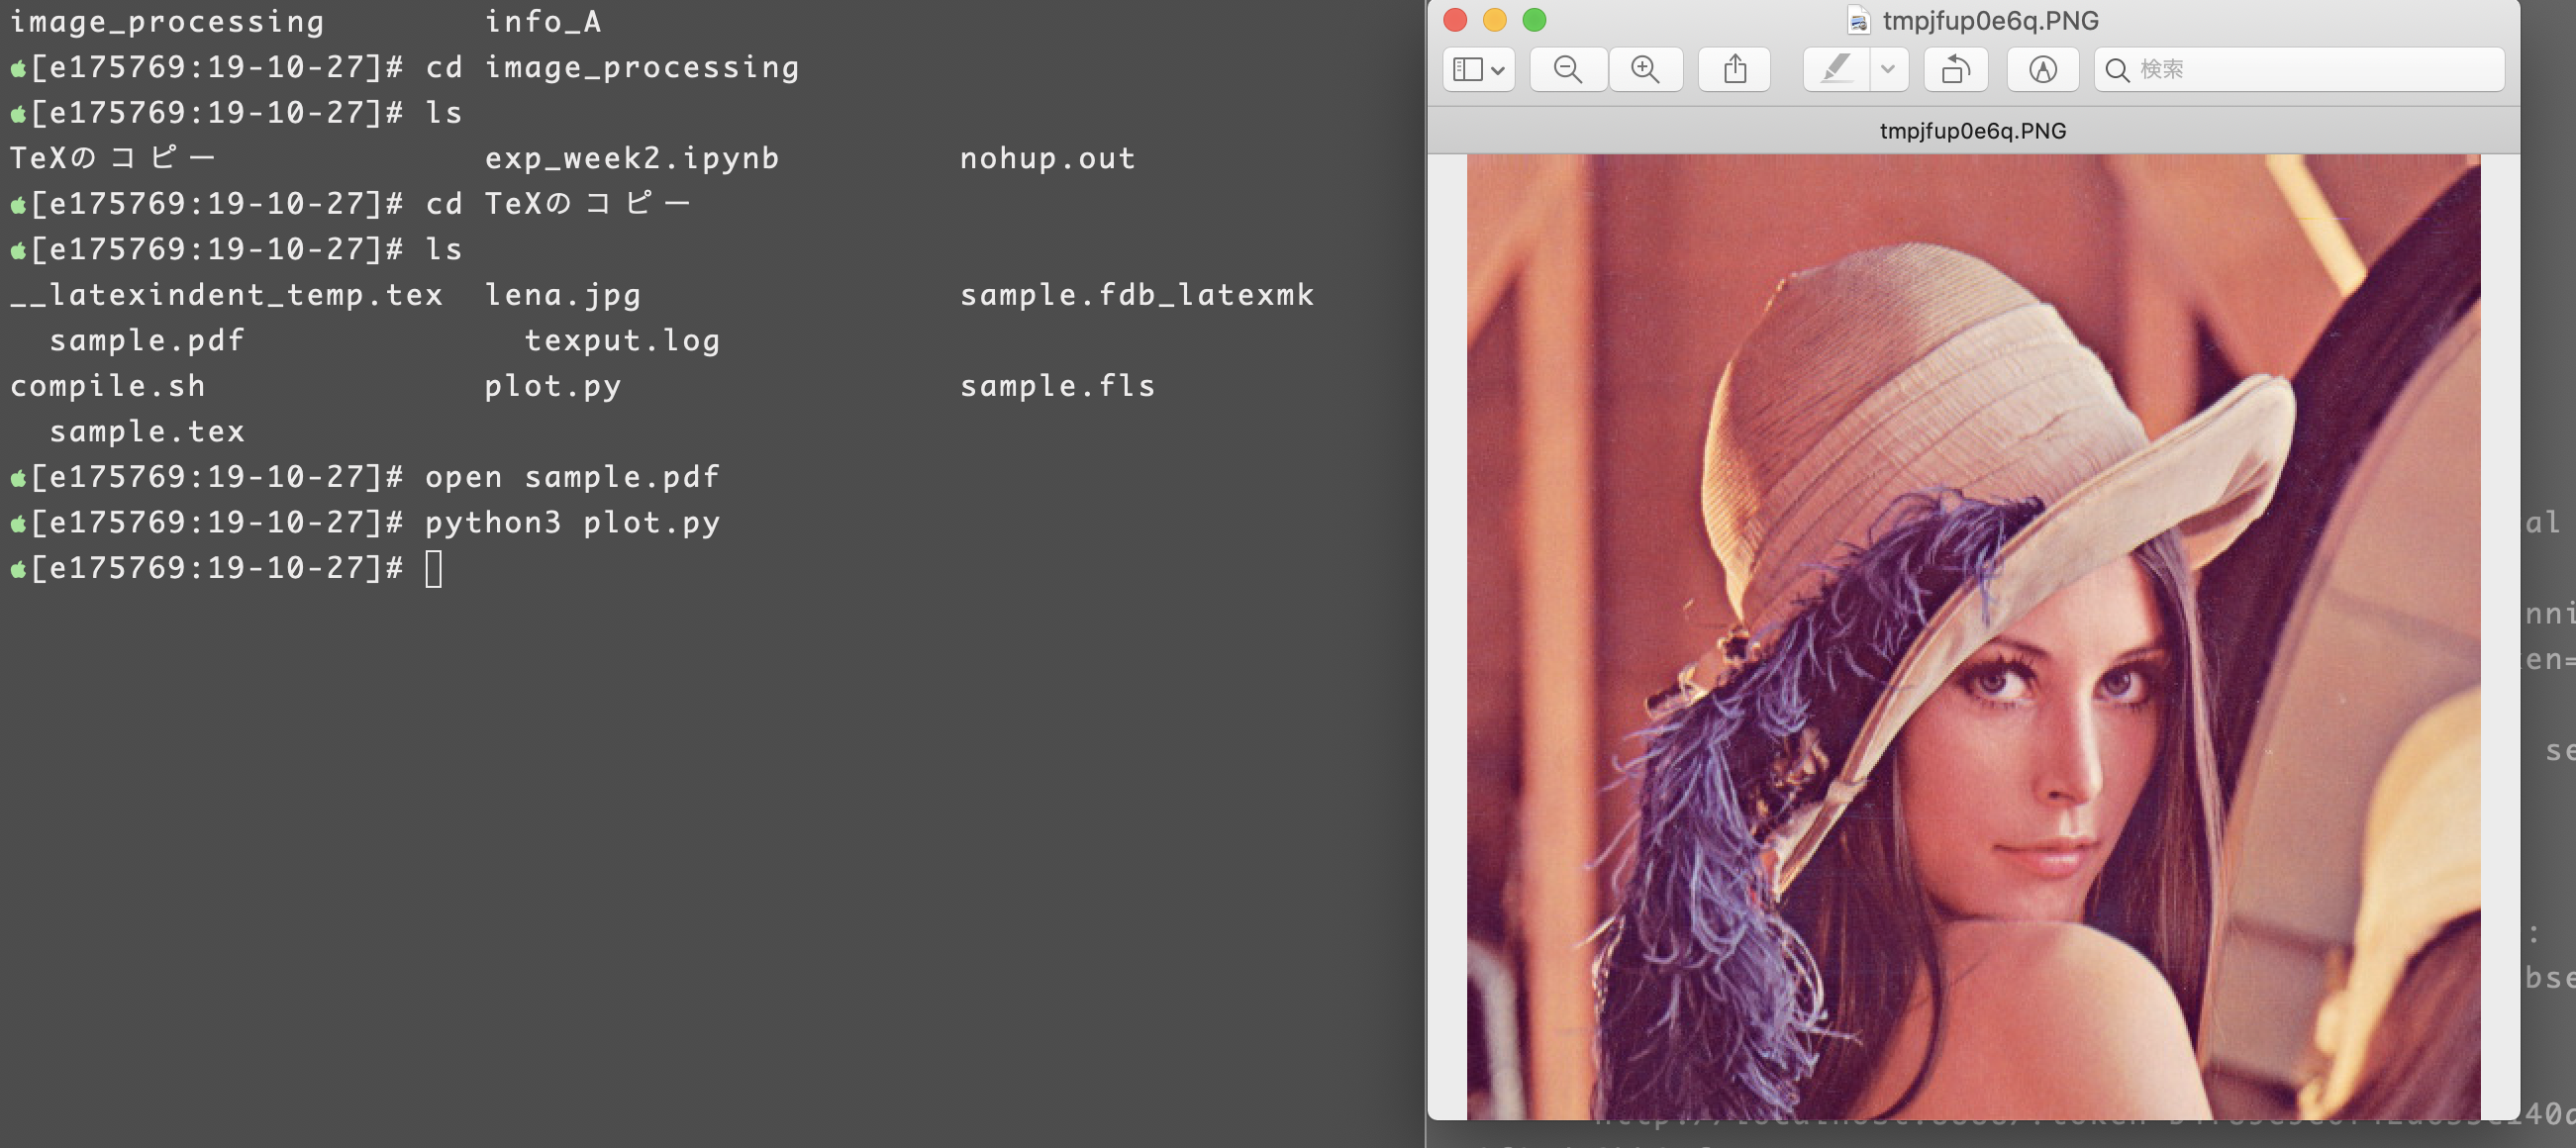
\includegraphics[width=120mm]{ex1.png}
	\caption{実行結果}
	\label{ex1}
\end{figure}
上記の図\ref{ex1}を参照するとPythonのコードを実行すると今回セットした画像が表示されていることがわかる。
%\lstinputlisting[numbers=left,breaklines=true,basicstyle=\ttfamily
%\footnotesize,frame=single,caption=サンプルプログラム,label=ex3]
%{ex3.sh}\label{ex3}

%\begin{figure}[H]
%	\centering
%	\includegraphics[width=80mm]{FA.png}
%	\caption{全加算器}
%	\label{}
%\end{figure}


\end{document}
